% Created by tikzDevice version 0.12.6 on 2023-12-13 11:00:58
% !TEX encoding = UTF-8 Unicode
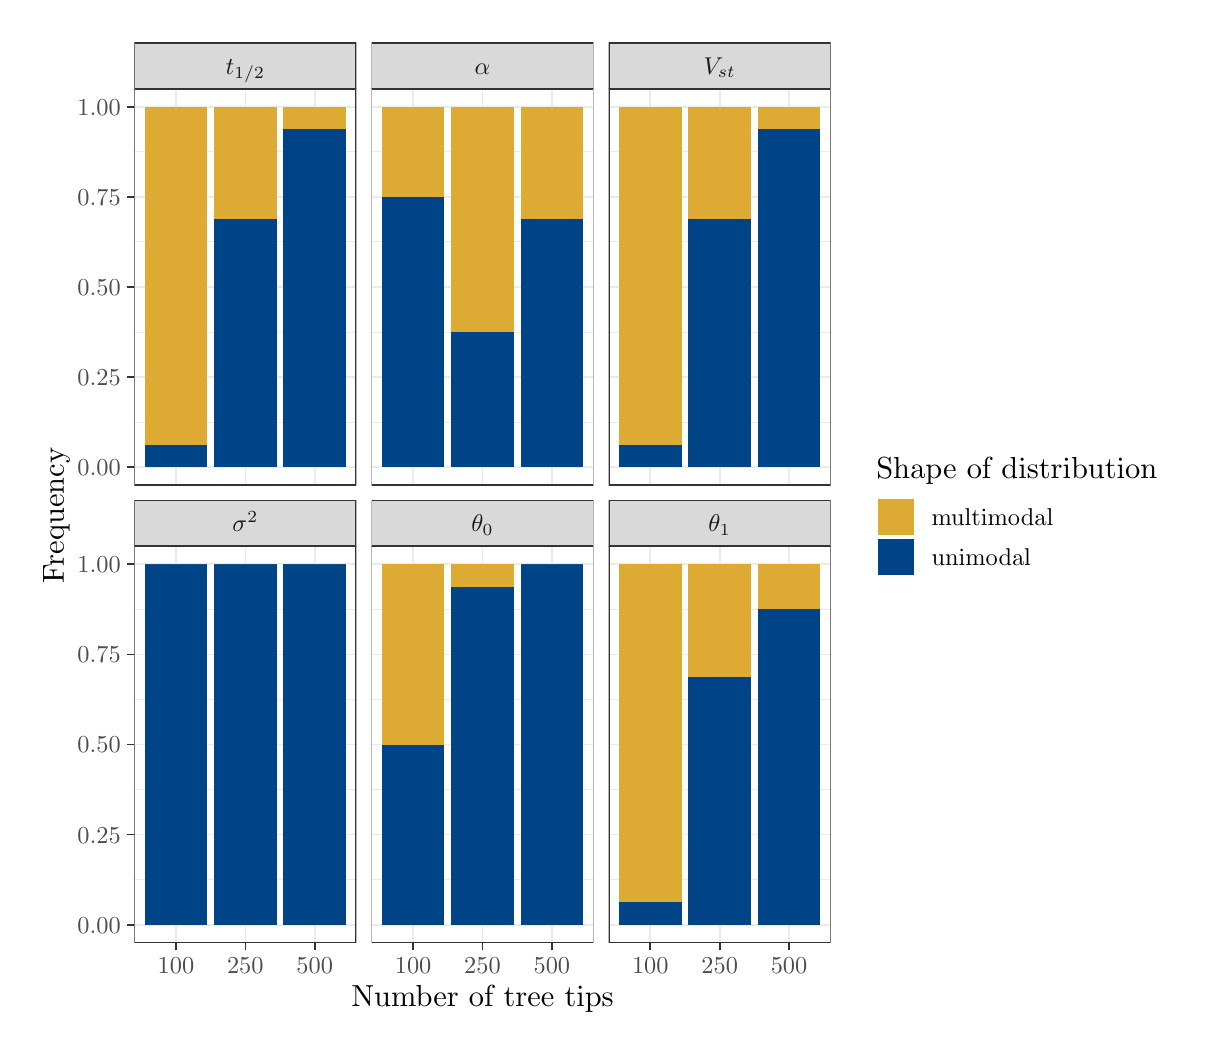
\begin{tikzpicture}[x=1pt,y=1pt]
\definecolor{fillColor}{RGB}{255,255,255}
\path[use as bounding box,fill=fillColor,fill opacity=0.00] (0,0) rectangle (419.17,361.35);
\begin{scope}
\path[clip] (  0.00,  0.00) rectangle (419.17,361.35);
\definecolor{drawColor}{RGB}{255,255,255}
\definecolor{fillColor}{RGB}{255,255,255}

\path[draw=drawColor,line width= 0.6pt,line join=round,line cap=round,fill=fillColor] (  0.00,  0.00) rectangle (419.17,361.35);
\end{scope}
\begin{scope}
\path[clip] ( 38.56,196.02) rectangle (118.75,339.28);
\definecolor{fillColor}{RGB}{255,255,255}

\path[fill=fillColor] ( 38.56,196.02) rectangle (118.75,339.28);
\definecolor{drawColor}{gray}{0.92}

\path[draw=drawColor,line width= 0.3pt,line join=round] ( 38.56,218.81) --
	(118.75,218.81);

\path[draw=drawColor,line width= 0.3pt,line join=round] ( 38.56,251.37) --
	(118.75,251.37);

\path[draw=drawColor,line width= 0.3pt,line join=round] ( 38.56,283.93) --
	(118.75,283.93);

\path[draw=drawColor,line width= 0.3pt,line join=round] ( 38.56,316.49) --
	(118.75,316.49);

\path[draw=drawColor,line width= 0.6pt,line join=round] ( 38.56,202.53) --
	(118.75,202.53);

\path[draw=drawColor,line width= 0.6pt,line join=round] ( 38.56,235.09) --
	(118.75,235.09);

\path[draw=drawColor,line width= 0.6pt,line join=round] ( 38.56,267.65) --
	(118.75,267.65);

\path[draw=drawColor,line width= 0.6pt,line join=round] ( 38.56,300.21) --
	(118.75,300.21);

\path[draw=drawColor,line width= 0.6pt,line join=round] ( 38.56,332.77) --
	(118.75,332.77);

\path[draw=drawColor,line width= 0.6pt,line join=round] ( 53.59,196.02) --
	( 53.59,339.28);

\path[draw=drawColor,line width= 0.6pt,line join=round] ( 78.65,196.02) --
	( 78.65,339.28);

\path[draw=drawColor,line width= 0.6pt,line join=round] (103.72,196.02) --
	(103.72,339.28);
\definecolor{fillColor}{RGB}{0,68,136}

\path[fill=fillColor] ( 42.31,202.53) rectangle ( 64.87,210.67);
\definecolor{fillColor}{RGB}{221,170,51}

\path[fill=fillColor] ( 42.31,210.67) rectangle ( 64.87,332.77);
\definecolor{fillColor}{RGB}{0,68,136}

\path[fill=fillColor] ( 67.38,202.53) rectangle ( 89.93,292.07);
\definecolor{fillColor}{RGB}{221,170,51}

\path[fill=fillColor] ( 67.38,292.07) rectangle ( 89.93,332.77);
\definecolor{fillColor}{RGB}{0,68,136}

\path[fill=fillColor] ( 92.44,202.53) rectangle (115.00,324.63);
\definecolor{fillColor}{RGB}{221,170,51}

\path[fill=fillColor] ( 92.44,324.63) rectangle (115.00,332.77);
\definecolor{drawColor}{gray}{0.20}

\path[draw=drawColor,line width= 0.6pt,line join=round,line cap=round] ( 38.56,196.02) rectangle (118.75,339.28);
\end{scope}
\begin{scope}
\path[clip] ( 38.56, 30.69) rectangle (118.75,173.95);
\definecolor{fillColor}{RGB}{255,255,255}

\path[fill=fillColor] ( 38.56, 30.69) rectangle (118.75,173.95);
\definecolor{drawColor}{gray}{0.92}

\path[draw=drawColor,line width= 0.3pt,line join=round] ( 38.56, 53.48) --
	(118.75, 53.48);

\path[draw=drawColor,line width= 0.3pt,line join=round] ( 38.56, 86.04) --
	(118.75, 86.04);

\path[draw=drawColor,line width= 0.3pt,line join=round] ( 38.56,118.60) --
	(118.75,118.60);

\path[draw=drawColor,line width= 0.3pt,line join=round] ( 38.56,151.15) --
	(118.75,151.15);

\path[draw=drawColor,line width= 0.6pt,line join=round] ( 38.56, 37.20) --
	(118.75, 37.20);

\path[draw=drawColor,line width= 0.6pt,line join=round] ( 38.56, 69.76) --
	(118.75, 69.76);

\path[draw=drawColor,line width= 0.6pt,line join=round] ( 38.56,102.32) --
	(118.75,102.32);

\path[draw=drawColor,line width= 0.6pt,line join=round] ( 38.56,134.88) --
	(118.75,134.88);

\path[draw=drawColor,line width= 0.6pt,line join=round] ( 38.56,167.43) --
	(118.75,167.43);

\path[draw=drawColor,line width= 0.6pt,line join=round] ( 53.59, 30.69) --
	( 53.59,173.95);

\path[draw=drawColor,line width= 0.6pt,line join=round] ( 78.65, 30.69) --
	( 78.65,173.95);

\path[draw=drawColor,line width= 0.6pt,line join=round] (103.72, 30.69) --
	(103.72,173.95);
\definecolor{fillColor}{RGB}{0,68,136}

\path[fill=fillColor] ( 42.31, 37.20) rectangle ( 64.87,167.43);
\definecolor{fillColor}{RGB}{221,170,51}

\path[fill=fillColor] ( 42.31,167.43) rectangle ( 64.87,167.43);
\definecolor{fillColor}{RGB}{0,68,136}

\path[fill=fillColor] ( 67.38, 37.20) rectangle ( 89.93,167.43);
\definecolor{fillColor}{RGB}{221,170,51}

\path[fill=fillColor] ( 67.38,167.43) rectangle ( 89.93,167.43);
\definecolor{fillColor}{RGB}{0,68,136}

\path[fill=fillColor] ( 92.44, 37.20) rectangle (115.00,167.43);
\definecolor{fillColor}{RGB}{221,170,51}

\path[fill=fillColor] ( 92.44,167.43) rectangle (115.00,167.43);
\definecolor{drawColor}{gray}{0.20}

\path[draw=drawColor,line width= 0.6pt,line join=round,line cap=round] ( 38.56, 30.69) rectangle (118.75,173.95);
\end{scope}
\begin{scope}
\path[clip] (124.25,196.02) rectangle (204.45,339.28);
\definecolor{fillColor}{RGB}{255,255,255}

\path[fill=fillColor] (124.25,196.02) rectangle (204.45,339.28);
\definecolor{drawColor}{gray}{0.92}

\path[draw=drawColor,line width= 0.3pt,line join=round] (124.25,218.81) --
	(204.45,218.81);

\path[draw=drawColor,line width= 0.3pt,line join=round] (124.25,251.37) --
	(204.45,251.37);

\path[draw=drawColor,line width= 0.3pt,line join=round] (124.25,283.93) --
	(204.45,283.93);

\path[draw=drawColor,line width= 0.3pt,line join=round] (124.25,316.49) --
	(204.45,316.49);

\path[draw=drawColor,line width= 0.6pt,line join=round] (124.25,202.53) --
	(204.45,202.53);

\path[draw=drawColor,line width= 0.6pt,line join=round] (124.25,235.09) --
	(204.45,235.09);

\path[draw=drawColor,line width= 0.6pt,line join=round] (124.25,267.65) --
	(204.45,267.65);

\path[draw=drawColor,line width= 0.6pt,line join=round] (124.25,300.21) --
	(204.45,300.21);

\path[draw=drawColor,line width= 0.6pt,line join=round] (124.25,332.77) --
	(204.45,332.77);

\path[draw=drawColor,line width= 0.6pt,line join=round] (139.29,196.02) --
	(139.29,339.28);

\path[draw=drawColor,line width= 0.6pt,line join=round] (164.35,196.02) --
	(164.35,339.28);

\path[draw=drawColor,line width= 0.6pt,line join=round] (189.42,196.02) --
	(189.42,339.28);
\definecolor{fillColor}{RGB}{0,68,136}

\path[fill=fillColor] (128.01,202.53) rectangle (150.57,300.21);
\definecolor{fillColor}{RGB}{221,170,51}

\path[fill=fillColor] (128.01,300.21) rectangle (150.57,332.77);
\definecolor{fillColor}{RGB}{0,68,136}

\path[fill=fillColor] (153.08,202.53) rectangle (175.63,251.37);
\definecolor{fillColor}{RGB}{221,170,51}

\path[fill=fillColor] (153.08,251.37) rectangle (175.63,332.77);
\definecolor{fillColor}{RGB}{0,68,136}

\path[fill=fillColor] (178.14,202.53) rectangle (200.70,292.07);
\definecolor{fillColor}{RGB}{221,170,51}

\path[fill=fillColor] (178.14,292.07) rectangle (200.70,332.77);
\definecolor{drawColor}{gray}{0.20}

\path[draw=drawColor,line width= 0.6pt,line join=round,line cap=round] (124.25,196.02) rectangle (204.45,339.28);
\end{scope}
\begin{scope}
\path[clip] (124.25, 30.69) rectangle (204.45,173.95);
\definecolor{fillColor}{RGB}{255,255,255}

\path[fill=fillColor] (124.25, 30.69) rectangle (204.45,173.95);
\definecolor{drawColor}{gray}{0.92}

\path[draw=drawColor,line width= 0.3pt,line join=round] (124.25, 53.48) --
	(204.45, 53.48);

\path[draw=drawColor,line width= 0.3pt,line join=round] (124.25, 86.04) --
	(204.45, 86.04);

\path[draw=drawColor,line width= 0.3pt,line join=round] (124.25,118.60) --
	(204.45,118.60);

\path[draw=drawColor,line width= 0.3pt,line join=round] (124.25,151.15) --
	(204.45,151.15);

\path[draw=drawColor,line width= 0.6pt,line join=round] (124.25, 37.20) --
	(204.45, 37.20);

\path[draw=drawColor,line width= 0.6pt,line join=round] (124.25, 69.76) --
	(204.45, 69.76);

\path[draw=drawColor,line width= 0.6pt,line join=round] (124.25,102.32) --
	(204.45,102.32);

\path[draw=drawColor,line width= 0.6pt,line join=round] (124.25,134.88) --
	(204.45,134.88);

\path[draw=drawColor,line width= 0.6pt,line join=round] (124.25,167.43) --
	(204.45,167.43);

\path[draw=drawColor,line width= 0.6pt,line join=round] (139.29, 30.69) --
	(139.29,173.95);

\path[draw=drawColor,line width= 0.6pt,line join=round] (164.35, 30.69) --
	(164.35,173.95);

\path[draw=drawColor,line width= 0.6pt,line join=round] (189.42, 30.69) --
	(189.42,173.95);
\definecolor{fillColor}{RGB}{0,68,136}

\path[fill=fillColor] (128.01, 37.20) rectangle (150.57,102.32);
\definecolor{fillColor}{RGB}{221,170,51}

\path[fill=fillColor] (128.01,102.32) rectangle (150.57,167.43);
\definecolor{fillColor}{RGB}{0,68,136}

\path[fill=fillColor] (153.08, 37.20) rectangle (175.63,159.29);
\definecolor{fillColor}{RGB}{221,170,51}

\path[fill=fillColor] (153.08,159.29) rectangle (175.63,167.43);
\definecolor{fillColor}{RGB}{0,68,136}

\path[fill=fillColor] (178.14, 37.20) rectangle (200.70,167.43);
\definecolor{fillColor}{RGB}{221,170,51}

\path[fill=fillColor] (178.14,167.43) rectangle (200.70,167.43);
\definecolor{drawColor}{gray}{0.20}

\path[draw=drawColor,line width= 0.6pt,line join=round,line cap=round] (124.25, 30.69) rectangle (204.45,173.95);
\end{scope}
\begin{scope}
\path[clip] (209.95,196.02) rectangle (290.15,339.28);
\definecolor{fillColor}{RGB}{255,255,255}

\path[fill=fillColor] (209.95,196.02) rectangle (290.15,339.28);
\definecolor{drawColor}{gray}{0.92}

\path[draw=drawColor,line width= 0.3pt,line join=round] (209.95,218.81) --
	(290.15,218.81);

\path[draw=drawColor,line width= 0.3pt,line join=round] (209.95,251.37) --
	(290.15,251.37);

\path[draw=drawColor,line width= 0.3pt,line join=round] (209.95,283.93) --
	(290.15,283.93);

\path[draw=drawColor,line width= 0.3pt,line join=round] (209.95,316.49) --
	(290.15,316.49);

\path[draw=drawColor,line width= 0.6pt,line join=round] (209.95,202.53) --
	(290.15,202.53);

\path[draw=drawColor,line width= 0.6pt,line join=round] (209.95,235.09) --
	(290.15,235.09);

\path[draw=drawColor,line width= 0.6pt,line join=round] (209.95,267.65) --
	(290.15,267.65);

\path[draw=drawColor,line width= 0.6pt,line join=round] (209.95,300.21) --
	(290.15,300.21);

\path[draw=drawColor,line width= 0.6pt,line join=round] (209.95,332.77) --
	(290.15,332.77);

\path[draw=drawColor,line width= 0.6pt,line join=round] (224.99,196.02) --
	(224.99,339.28);

\path[draw=drawColor,line width= 0.6pt,line join=round] (250.05,196.02) --
	(250.05,339.28);

\path[draw=drawColor,line width= 0.6pt,line join=round] (275.12,196.02) --
	(275.12,339.28);
\definecolor{fillColor}{RGB}{0,68,136}

\path[fill=fillColor] (213.71,202.53) rectangle (236.27,210.67);
\definecolor{fillColor}{RGB}{221,170,51}

\path[fill=fillColor] (213.71,210.67) rectangle (236.27,332.77);
\definecolor{fillColor}{RGB}{0,68,136}

\path[fill=fillColor] (238.78,202.53) rectangle (261.33,292.07);
\definecolor{fillColor}{RGB}{221,170,51}

\path[fill=fillColor] (238.78,292.07) rectangle (261.33,332.77);
\definecolor{fillColor}{RGB}{0,68,136}

\path[fill=fillColor] (263.84,202.53) rectangle (286.39,324.63);
\definecolor{fillColor}{RGB}{221,170,51}

\path[fill=fillColor] (263.84,324.63) rectangle (286.39,332.77);
\definecolor{drawColor}{gray}{0.20}

\path[draw=drawColor,line width= 0.6pt,line join=round,line cap=round] (209.95,196.02) rectangle (290.15,339.28);
\end{scope}
\begin{scope}
\path[clip] (209.95, 30.69) rectangle (290.15,173.95);
\definecolor{fillColor}{RGB}{255,255,255}

\path[fill=fillColor] (209.95, 30.69) rectangle (290.15,173.95);
\definecolor{drawColor}{gray}{0.92}

\path[draw=drawColor,line width= 0.3pt,line join=round] (209.95, 53.48) --
	(290.15, 53.48);

\path[draw=drawColor,line width= 0.3pt,line join=round] (209.95, 86.04) --
	(290.15, 86.04);

\path[draw=drawColor,line width= 0.3pt,line join=round] (209.95,118.60) --
	(290.15,118.60);

\path[draw=drawColor,line width= 0.3pt,line join=round] (209.95,151.15) --
	(290.15,151.15);

\path[draw=drawColor,line width= 0.6pt,line join=round] (209.95, 37.20) --
	(290.15, 37.20);

\path[draw=drawColor,line width= 0.6pt,line join=round] (209.95, 69.76) --
	(290.15, 69.76);

\path[draw=drawColor,line width= 0.6pt,line join=round] (209.95,102.32) --
	(290.15,102.32);

\path[draw=drawColor,line width= 0.6pt,line join=round] (209.95,134.88) --
	(290.15,134.88);

\path[draw=drawColor,line width= 0.6pt,line join=round] (209.95,167.43) --
	(290.15,167.43);

\path[draw=drawColor,line width= 0.6pt,line join=round] (224.99, 30.69) --
	(224.99,173.95);

\path[draw=drawColor,line width= 0.6pt,line join=round] (250.05, 30.69) --
	(250.05,173.95);

\path[draw=drawColor,line width= 0.6pt,line join=round] (275.12, 30.69) --
	(275.12,173.95);
\definecolor{fillColor}{RGB}{0,68,136}

\path[fill=fillColor] (213.71, 37.20) rectangle (236.27, 45.34);
\definecolor{fillColor}{RGB}{221,170,51}

\path[fill=fillColor] (213.71, 45.34) rectangle (236.27,167.43);
\definecolor{fillColor}{RGB}{0,68,136}

\path[fill=fillColor] (238.78, 37.20) rectangle (261.33,126.74);
\definecolor{fillColor}{RGB}{221,170,51}

\path[fill=fillColor] (238.78,126.74) rectangle (261.33,167.43);
\definecolor{fillColor}{RGB}{0,68,136}

\path[fill=fillColor] (263.84, 37.20) rectangle (286.39,151.15);
\definecolor{fillColor}{RGB}{221,170,51}

\path[fill=fillColor] (263.84,151.15) rectangle (286.39,167.43);
\definecolor{drawColor}{gray}{0.20}

\path[draw=drawColor,line width= 0.6pt,line join=round,line cap=round] (209.95, 30.69) rectangle (290.15,173.95);
\end{scope}
\begin{scope}
\path[clip] ( 38.56,173.95) rectangle (118.75,190.52);
\definecolor{drawColor}{gray}{0.20}
\definecolor{fillColor}{gray}{0.85}

\path[draw=drawColor,line width= 0.6pt,line join=round,line cap=round,fill=fillColor] ( 38.56,173.95) rectangle (118.75,190.52);
\definecolor{drawColor}{gray}{0.10}

\node[text=drawColor,anchor=base,inner sep=0pt, outer sep=0pt, scale=  0.88] at ( 78.65,179.20) {$\sigma^2$};
\end{scope}
\begin{scope}
\path[clip] (124.25,173.95) rectangle (204.45,190.52);
\definecolor{drawColor}{gray}{0.20}
\definecolor{fillColor}{gray}{0.85}

\path[draw=drawColor,line width= 0.6pt,line join=round,line cap=round,fill=fillColor] (124.25,173.95) rectangle (204.45,190.52);
\definecolor{drawColor}{gray}{0.10}

\node[text=drawColor,anchor=base,inner sep=0pt, outer sep=0pt, scale=  0.88] at (164.35,179.20) {$\theta_0$};
\end{scope}
\begin{scope}
\path[clip] (209.95,173.95) rectangle (290.15,190.52);
\definecolor{drawColor}{gray}{0.20}
\definecolor{fillColor}{gray}{0.85}

\path[draw=drawColor,line width= 0.6pt,line join=round,line cap=round,fill=fillColor] (209.95,173.95) rectangle (290.15,190.52);
\definecolor{drawColor}{gray}{0.10}

\node[text=drawColor,anchor=base,inner sep=0pt, outer sep=0pt, scale=  0.88] at (250.05,179.20) {$\theta_1$};
\end{scope}
\begin{scope}
\path[clip] ( 38.56,339.28) rectangle (118.75,355.85);
\definecolor{drawColor}{gray}{0.20}
\definecolor{fillColor}{gray}{0.85}

\path[draw=drawColor,line width= 0.6pt,line join=round,line cap=round,fill=fillColor] ( 38.56,339.28) rectangle (118.75,355.85);
\definecolor{drawColor}{gray}{0.10}

\node[text=drawColor,anchor=base,inner sep=0pt, outer sep=0pt, scale=  0.88] at ( 78.65,344.53) {$t_{1/2}$};
\end{scope}
\begin{scope}
\path[clip] (124.25,339.28) rectangle (204.45,355.85);
\definecolor{drawColor}{gray}{0.20}
\definecolor{fillColor}{gray}{0.85}

\path[draw=drawColor,line width= 0.6pt,line join=round,line cap=round,fill=fillColor] (124.25,339.28) rectangle (204.45,355.85);
\definecolor{drawColor}{gray}{0.10}

\node[text=drawColor,anchor=base,inner sep=0pt, outer sep=0pt, scale=  0.88] at (164.35,344.53) {$\alpha$};
\end{scope}
\begin{scope}
\path[clip] (209.95,339.28) rectangle (290.15,355.85);
\definecolor{drawColor}{gray}{0.20}
\definecolor{fillColor}{gray}{0.85}

\path[draw=drawColor,line width= 0.6pt,line join=round,line cap=round,fill=fillColor] (209.95,339.28) rectangle (290.15,355.85);
\definecolor{drawColor}{gray}{0.10}

\node[text=drawColor,anchor=base,inner sep=0pt, outer sep=0pt, scale=  0.88] at (250.05,344.53) {$V_{st}$};
\end{scope}
\begin{scope}
\path[clip] (  0.00,  0.00) rectangle (419.17,361.35);
\definecolor{drawColor}{gray}{0.20}

\path[draw=drawColor,line width= 0.6pt,line join=round] ( 53.59, 27.94) --
	( 53.59, 30.69);

\path[draw=drawColor,line width= 0.6pt,line join=round] ( 78.65, 27.94) --
	( 78.65, 30.69);

\path[draw=drawColor,line width= 0.6pt,line join=round] (103.72, 27.94) --
	(103.72, 30.69);
\end{scope}
\begin{scope}
\path[clip] (  0.00,  0.00) rectangle (419.17,361.35);
\definecolor{drawColor}{gray}{0.30}

\node[text=drawColor,anchor=base,inner sep=0pt, outer sep=0pt, scale=  0.88] at ( 53.59, 19.68) {100};

\node[text=drawColor,anchor=base,inner sep=0pt, outer sep=0pt, scale=  0.88] at ( 78.65, 19.68) {250};

\node[text=drawColor,anchor=base,inner sep=0pt, outer sep=0pt, scale=  0.88] at (103.72, 19.68) {500};
\end{scope}
\begin{scope}
\path[clip] (  0.00,  0.00) rectangle (419.17,361.35);
\definecolor{drawColor}{gray}{0.20}

\path[draw=drawColor,line width= 0.6pt,line join=round] (139.29, 27.94) --
	(139.29, 30.69);

\path[draw=drawColor,line width= 0.6pt,line join=round] (164.35, 27.94) --
	(164.35, 30.69);

\path[draw=drawColor,line width= 0.6pt,line join=round] (189.42, 27.94) --
	(189.42, 30.69);
\end{scope}
\begin{scope}
\path[clip] (  0.00,  0.00) rectangle (419.17,361.35);
\definecolor{drawColor}{gray}{0.30}

\node[text=drawColor,anchor=base,inner sep=0pt, outer sep=0pt, scale=  0.88] at (139.29, 19.68) {100};

\node[text=drawColor,anchor=base,inner sep=0pt, outer sep=0pt, scale=  0.88] at (164.35, 19.68) {250};

\node[text=drawColor,anchor=base,inner sep=0pt, outer sep=0pt, scale=  0.88] at (189.42, 19.68) {500};
\end{scope}
\begin{scope}
\path[clip] (  0.00,  0.00) rectangle (419.17,361.35);
\definecolor{drawColor}{gray}{0.20}

\path[draw=drawColor,line width= 0.6pt,line join=round] (224.99, 27.94) --
	(224.99, 30.69);

\path[draw=drawColor,line width= 0.6pt,line join=round] (250.05, 27.94) --
	(250.05, 30.69);

\path[draw=drawColor,line width= 0.6pt,line join=round] (275.12, 27.94) --
	(275.12, 30.69);
\end{scope}
\begin{scope}
\path[clip] (  0.00,  0.00) rectangle (419.17,361.35);
\definecolor{drawColor}{gray}{0.30}

\node[text=drawColor,anchor=base,inner sep=0pt, outer sep=0pt, scale=  0.88] at (224.99, 19.68) {100};

\node[text=drawColor,anchor=base,inner sep=0pt, outer sep=0pt, scale=  0.88] at (250.05, 19.68) {250};

\node[text=drawColor,anchor=base,inner sep=0pt, outer sep=0pt, scale=  0.88] at (275.12, 19.68) {500};
\end{scope}
\begin{scope}
\path[clip] (  0.00,  0.00) rectangle (419.17,361.35);
\definecolor{drawColor}{gray}{0.30}

\node[text=drawColor,anchor=base east,inner sep=0pt, outer sep=0pt, scale=  0.88] at ( 33.61,199.50) {0.00};

\node[text=drawColor,anchor=base east,inner sep=0pt, outer sep=0pt, scale=  0.88] at ( 33.61,232.06) {0.25};

\node[text=drawColor,anchor=base east,inner sep=0pt, outer sep=0pt, scale=  0.88] at ( 33.61,264.62) {0.50};

\node[text=drawColor,anchor=base east,inner sep=0pt, outer sep=0pt, scale=  0.88] at ( 33.61,297.18) {0.75};

\node[text=drawColor,anchor=base east,inner sep=0pt, outer sep=0pt, scale=  0.88] at ( 33.61,329.74) {1.00};
\end{scope}
\begin{scope}
\path[clip] (  0.00,  0.00) rectangle (419.17,361.35);
\definecolor{drawColor}{gray}{0.20}

\path[draw=drawColor,line width= 0.6pt,line join=round] ( 35.81,202.53) --
	( 38.56,202.53);

\path[draw=drawColor,line width= 0.6pt,line join=round] ( 35.81,235.09) --
	( 38.56,235.09);

\path[draw=drawColor,line width= 0.6pt,line join=round] ( 35.81,267.65) --
	( 38.56,267.65);

\path[draw=drawColor,line width= 0.6pt,line join=round] ( 35.81,300.21) --
	( 38.56,300.21);

\path[draw=drawColor,line width= 0.6pt,line join=round] ( 35.81,332.77) --
	( 38.56,332.77);
\end{scope}
\begin{scope}
\path[clip] (  0.00,  0.00) rectangle (419.17,361.35);
\definecolor{drawColor}{gray}{0.30}

\node[text=drawColor,anchor=base east,inner sep=0pt, outer sep=0pt, scale=  0.88] at ( 33.61, 34.17) {0.00};

\node[text=drawColor,anchor=base east,inner sep=0pt, outer sep=0pt, scale=  0.88] at ( 33.61, 66.73) {0.25};

\node[text=drawColor,anchor=base east,inner sep=0pt, outer sep=0pt, scale=  0.88] at ( 33.61, 99.29) {0.50};

\node[text=drawColor,anchor=base east,inner sep=0pt, outer sep=0pt, scale=  0.88] at ( 33.61,131.84) {0.75};

\node[text=drawColor,anchor=base east,inner sep=0pt, outer sep=0pt, scale=  0.88] at ( 33.61,164.40) {1.00};
\end{scope}
\begin{scope}
\path[clip] (  0.00,  0.00) rectangle (419.17,361.35);
\definecolor{drawColor}{gray}{0.20}

\path[draw=drawColor,line width= 0.6pt,line join=round] ( 35.81, 37.20) --
	( 38.56, 37.20);

\path[draw=drawColor,line width= 0.6pt,line join=round] ( 35.81, 69.76) --
	( 38.56, 69.76);

\path[draw=drawColor,line width= 0.6pt,line join=round] ( 35.81,102.32) --
	( 38.56,102.32);

\path[draw=drawColor,line width= 0.6pt,line join=round] ( 35.81,134.88) --
	( 38.56,134.88);

\path[draw=drawColor,line width= 0.6pt,line join=round] ( 35.81,167.43) --
	( 38.56,167.43);
\end{scope}
\begin{scope}
\path[clip] (  0.00,  0.00) rectangle (419.17,361.35);
\definecolor{drawColor}{RGB}{0,0,0}

\node[text=drawColor,anchor=base,inner sep=0pt, outer sep=0pt, scale=  1.10] at (164.35,  7.64) {Number of tree tips};
\end{scope}
\begin{scope}
\path[clip] (  0.00,  0.00) rectangle (419.17,361.35);
\definecolor{drawColor}{RGB}{0,0,0}

\node[text=drawColor,rotate= 90.00,anchor=base,inner sep=0pt, outer sep=0pt, scale=  1.10] at ( 13.08,184.98) {Frequency};
\end{scope}
\begin{scope}
\path[clip] (  0.00,  0.00) rectangle (419.17,361.35);
\definecolor{fillColor}{RGB}{255,255,255}

\path[fill=fillColor] (301.15,157.42) rectangle (413.67,212.54);
\end{scope}
\begin{scope}
\path[clip] (  0.00,  0.00) rectangle (419.17,361.35);
\definecolor{drawColor}{RGB}{0,0,0}

\node[text=drawColor,anchor=base west,inner sep=0pt, outer sep=0pt, scale=  1.10] at (306.65,198.40) {Shape of distribution};
\end{scope}
\begin{scope}
\path[clip] (  0.00,  0.00) rectangle (419.17,361.35);
\definecolor{fillColor}{RGB}{255,255,255}

\path[fill=fillColor] (306.65,177.37) rectangle (321.11,191.83);
\end{scope}
\begin{scope}
\path[clip] (  0.00,  0.00) rectangle (419.17,361.35);
\definecolor{fillColor}{RGB}{221,170,51}

\path[fill=fillColor] (307.37,178.09) rectangle (320.40,191.12);
\end{scope}
\begin{scope}
\path[clip] (  0.00,  0.00) rectangle (419.17,361.35);
\definecolor{fillColor}{RGB}{255,255,255}

\path[fill=fillColor] (306.65,162.92) rectangle (321.11,177.38);
\end{scope}
\begin{scope}
\path[clip] (  0.00,  0.00) rectangle (419.17,361.35);
\definecolor{fillColor}{RGB}{0,68,136}

\path[fill=fillColor] (307.37,163.63) rectangle (320.40,176.66);
\end{scope}
\begin{scope}
\path[clip] (  0.00,  0.00) rectangle (419.17,361.35);
\definecolor{drawColor}{RGB}{0,0,0}

\node[text=drawColor,anchor=base west,inner sep=0pt, outer sep=0pt, scale=  0.88] at (326.61,181.57) {multimodal};
\end{scope}
\begin{scope}
\path[clip] (  0.00,  0.00) rectangle (419.17,361.35);
\definecolor{drawColor}{RGB}{0,0,0}

\node[text=drawColor,anchor=base west,inner sep=0pt, outer sep=0pt, scale=  0.88] at (326.61,167.12) {unimodal};
\end{scope}
\end{tikzpicture}
